\section{Methods}
\lb{sec:methods}


The purpose of this section is to describe the ML methods that we use for the classification:
random forests, boosted decision trees, (simple decision trees?), neural networks, logistic regression, support vector machine.

Methodology
\ben
\item
Split the PS with known classification into learning and test samples.
\item
Use the learning sample for training and for selection of features.
In particular, continuous parameters, such as the thresholds in the decision trees or mixing matrices in neural networks, are determined from the leaning sample. 
\item
Meta-parameters, which encode the complexity of the methods, such as the depth of the decision trees,
are determined from the best performance on the test sample.
\een

\subsection{Details of the analysis}


In this subsection we give more details on the analysis:
\ben
\item
Describe the features that we use for the analysis.
\item
Describe the objective function for minimization (accuracy of classification on learning sample).
Weighted objective function: give more weight to pulsars, since there are fewer of them in the catalog.
\item
Learning curve using all features?
{\it Plot: classification accuracy using the total list of features for learning and test sample as a function of complexity parameter.}
\item
Selection of the most important features.
{\it Table: features vs algorithms. Columns: algorithms, rows: features, values: significance.}
\item
Selection of meta-parameters.
{\it Plot: classification results for the test sample using a subset of features.}
\item
Train the final classifier.
{\it Table: classification accuracy of the final classifiers for different algorithms using the test sample from 3FGL.}
\een

Discuss the general features of the optimal algorithms: which features turn out to be important, what is the depth of the trees, the number of trees in random forests, the depth and number of internal nodes in the neural networks. 

\begin{figure}[h]
%\centering
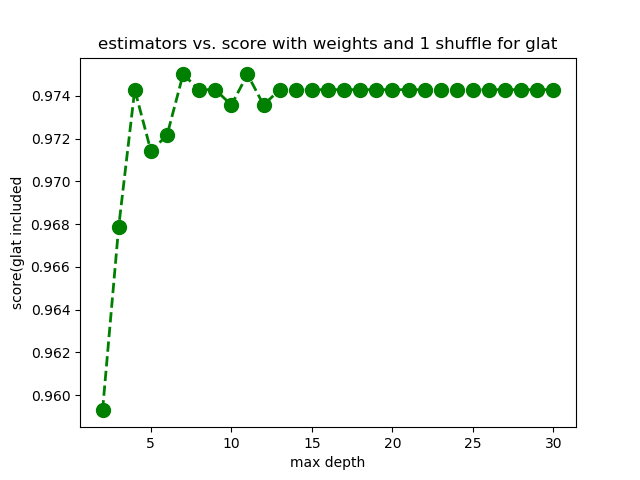
\includegraphics[width=\onepic\textwidth]{plots/Rf_maxdepth_oobscore_glat}
\caption{
Example of a figure for one column.
}
\label{fig:Maps_data}
\end{figure}


\begin{figure*}[h]
%\centering
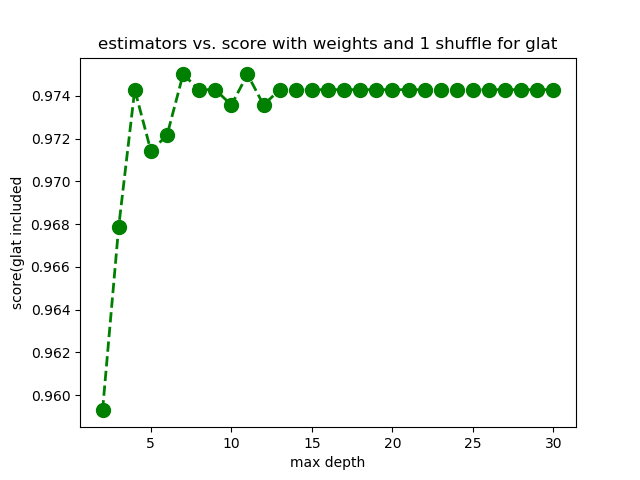
\includegraphics[width=\twopicsp\textwidth]{plots/Rf_maxdepth_oobscore_glat}
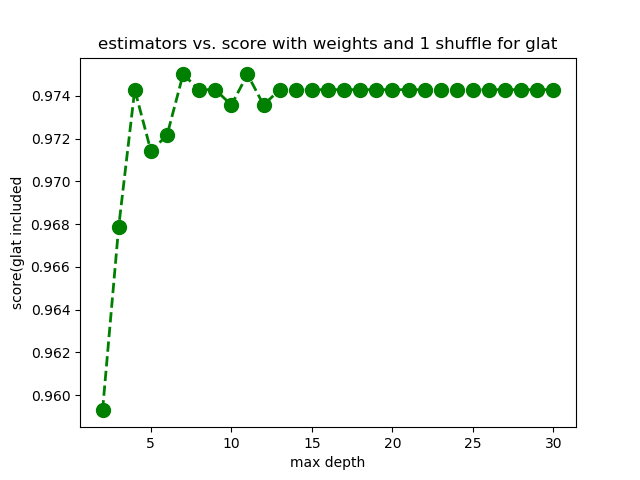
\includegraphics[width=\twopicsp\textwidth]{plots/Rf_maxdepth_oobscore_glat}
\caption{
Example of a figure for both columns.
}
\label{fig:Maps_data}
\end{figure*}


\subsection{Comparison of the classification algorithms}

{\it Plot: classification domains for a pair of features (or different pairs of features, e.g., latitude vs index, index vs curvature, latitude vs variability).}

Probabilistic classification? Result: probability for a source to belong to a particular class.
Result of classification: table of sources with probabilities for different algorithms.
Final probability: the probability for one of the algorithms (for the most precise one?) and uncertainties determined from the other algorithms.

Discuss a few examples where algorithms give different predictions (are these sources at the boundaries of the domains).

Discuss examples where algorithms misclassify sources from the test sample.




